\chapter{Device Background}\label{cha:device_background}

Before describing measurements at the focus of this thesis, it is important to first introduce the devices we use to engineer interesting states, and the tools we use to measure them. As an overview, we use a material called GaAs/AlGaAs heterostructure, the precise layering of the semiconductors form a two-dimensional electron gas (2DEG) below the surface of the heterostructure. Voltages applied to patterened metallic gates ontop of the heterostructre can control the electrons in the 2DEG allowing for the formation of quantum point contacts (QPCs) and quantum dots  (QDs). Ohmics are used to contact the 2DEG, allowing for transport measurements through such structures. 

\section{Two-Dimensional Electron Gas (2DEG)}



\begin{figure}[!htb]
  \begin{center}
%% psfrag: comment the following line if not using the psfrag package
    % \psfrag{pie makes me happy!}{$\pi$ makes me happy!}
%% includegraphics: comment the following if not using the graphicx package
    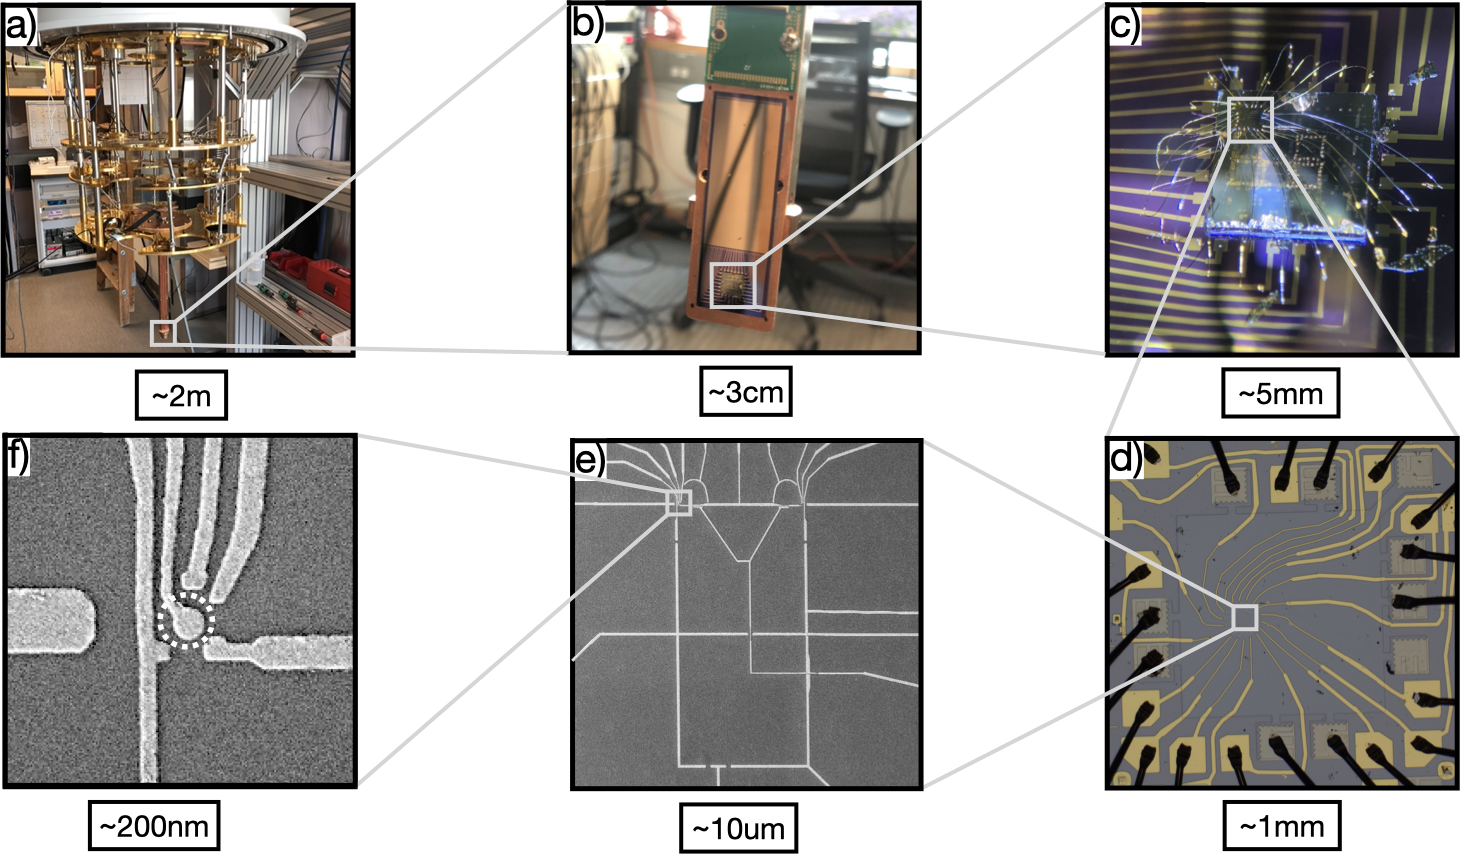
\includegraphics[width=1.0\textwidth]{figures/ch1/crop_PosterFiguresMaster.001.png}
    \caption[Two-dimensional electron gas in a GaAs/AlGaAs heterostructure]{\label{fig:ch1/2deg} 
    % For some options that work with pdf\LaTeX, please see this discussion:
    %   \url{http://tex.stackexchange.com/questions/11839}.  
    CAPTION TO BE ADDED. FIGURE TO BE CHANGED TOI HETEROSTRUCTURE.  
      }
  \end{center}
\end{figure}



The quantum point contacts (QPCs) and quantum dots (QDs) described later in this thesis are engineered in a two-dimensional electron gas (2DEG). A 2DEG can be thought of as a two dimensional plane of electrons which can move freely along the x and y direction, but are tightly confined in the z direction. The 2DEGs' in this thesis are realised in GaAs/AlGaAs heterostructures. A semiconductor heterostructure refers to a material system composed of two or more semiconductor materials with different bandgaps or lattice constants that are layered together Fig.~\ref{fig:ch1/2deg}. These layers are typically grown on top of each other using techniques such as molecular beam epitaxy (MBE). The heterostructures in this thesis are grown by Michael Manfra's lab at Purdue University [reference XXX]. 

There are two characteristics of this heterostructure which give rise to a 2DEG. Firstly, $\mathrm{Al_xGa_{1-x}As}$ has a tunable bandgap ranging from 1.42 - \qty{2.16}{eV} [REFERENCE XXX] whilst GaAs has a bandgap of \qty{1.42}{eV}. Secondly, an n-type dopant layer is sandwiched between the $\mathrm{Al_xGa_{1-x}As}$ layers. The smaller bandgap of GaAs allows the electrons from the donar atoms in the dopant layer to drop into the GaAs conduction band resulting in a triangular potential well. This triangular well contains of multiple sub-bands. The second sub-band is $\qty{\sim 150}{meV}$ above the first and will remain unoccupied as than energy gap is much greater than measurement temperatures $\qty{500}{mK}\sim\qty{43}{\mu eV}$ and source-drain bias $\qty{100}{\mu eV}$, hence, the electron gas can be considered two-dimensional.

Efforts are made to keep the heterostructure and 2DEG clean and defect free. A \qty{7}{nm} cap of GaAs is placed ontop of the heterostructure to prevent oxidation. A small lattice mis-match between the GaAs and AlGaAs layers keeps the number of boundary defects in the 2DEG plane low. The \qty{30}{nm} AlGaAs buffer layer between the 2DEG and dopants helps prevent defects near the 2DEG plane. The resulting 2DEGs' has a high mobility $\mathrm{\mu_e}~=~\qty{2.56e6}{cm^2/Vs}$ and electron density $\mathrm{n}~=~\qty{2.42e11}{cm^{-2}}$

Fabrication details on these devices `re described in Appendix [XXX]. As an overview, the heterostructure is divided into separate areas with isolated 2DEGs' by etching away the top layers of the heterostructure to remove the 2DEG. Contact to the 2DEG is made with ohmics contacts. These are made by annealing a layer of Ni-Au-Ge, the metal diffuses through the heterostructure and forms an electrical connection to the 2DEG. An insulating dielectric of \qty{10}{nm} $\mathrm{Al_2O_3}$ is deposited across the surface of the heterostructure to limit leakage from the metallic gates.  A thin layer (\qty{10}{nm}) of Au is deposited to form the inner gates which we design to form the QPCs and QDs. In a second step, a thick layer (\qty{100}{nm}) of Au is deposited (our outer gates) to connect the inner gates to square bond pads. Wire bonds are then made from chip carrier to the square bond pads which allows for connection between fridge wiring and the quantum device. 




\afterpage{\clearpage}
\section{Quantum Point Contact (QPC)}

\begin{figure}[!htb]
  \begin{center}
%% includegraphics: comment the following if not using the graphicx package
    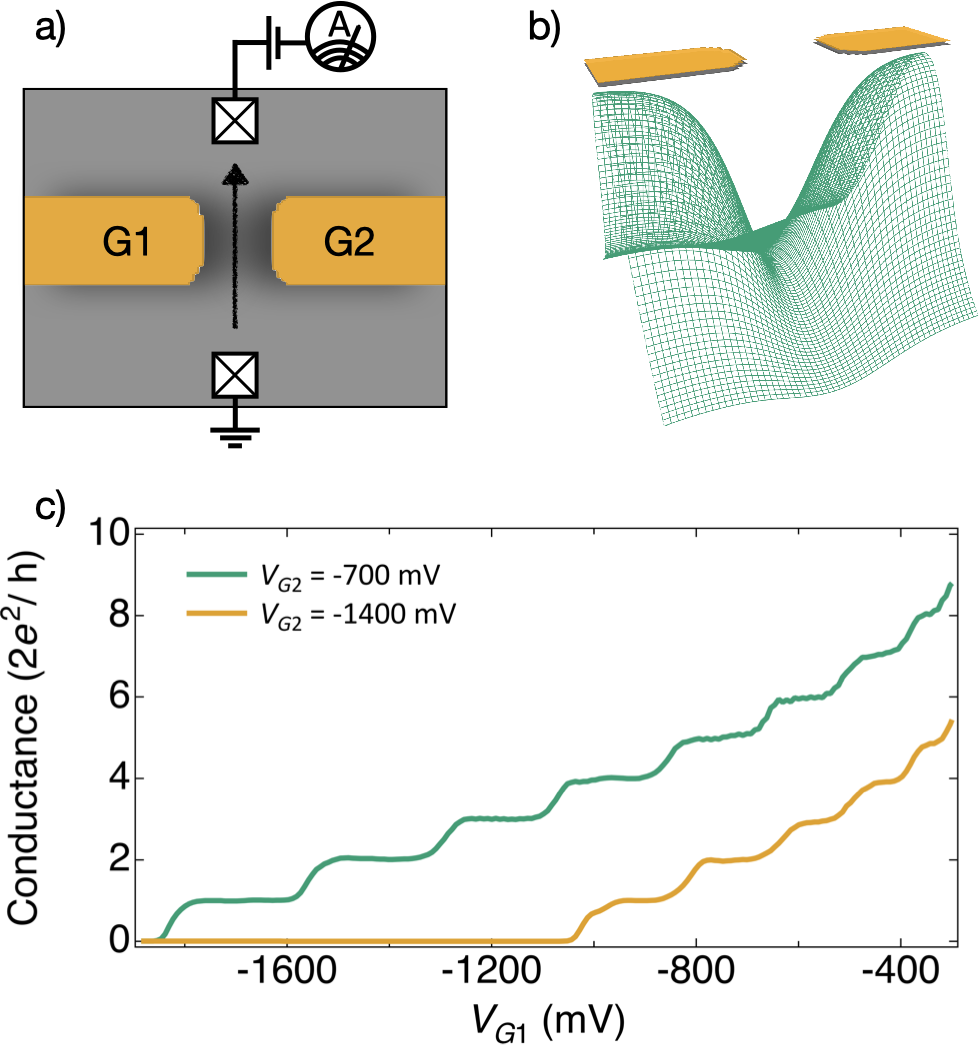
\includegraphics[width=0.9\textwidth]{figures/ch1/crop_PosterFiguresMaster.002.png}
    \caption[Conductance through a quantum point contact]{\label{fig:ch1/qpc_intro} 
    % For some options that work with pdf\LaTeX, please see this discussion:
    %   \url{http://tex.stackexchange.com/questions/11839}.  
    (\textbf{a}) A graphic representation from a top-down view of a quantum point contact (QPC). The gold fingers are the metallic gates where negative voltages can be applied to. The grey is where the electrons in the 2DEG can go dependant on the amount of negative voltage applied to the gates. The crossed squares are ohmic contacts to the 2DEG so that bias can be applied and the conductance through the QPC is measured. (\textbf{b}) is a representation of the electric potential the electrons see in the 2DEG due to negative voltage applied to the gates. With sufficient negative voltages applied to the gates, the electrons cannot overcome the potential barrier under the gate and flow through the middle. (\textbf{c}) is a measurement showing the quantised conductance through a QPC as the voltage on G1 becomes more negative. The voltage on the gates can be made negative enough so that electrons cannot tunnel across the potential barrier and hence we measure 0 conductance. 
      }
  \end{center}
\end{figure}

In this thesis a quantum point contact (QPC) is one-dimensional channel connected to a source and drain reservoir Fig.~\ref{fig:ch1/qpc_intro}. A one-dimensional channel in the 2DEG is engineered by putting sufficient negative voltage on metal gates deposited on the surface of the heterostructure. By applying a potential bias between the ohmics a current will flow. The more negative the voltage on the gate, the higher the potential barrier is for the electrons in the 2DEG. A large enough potential barrier can stop the electrons flowing underneath the gate (called 'depletion'), however, they can still flow between the gates. It normally requires a more negative voltage to stop electrons flowing between the gates (called 'pinch-off'). A QPC length is the length of the one-dimensional channel and the width is the empty space between gates. In our devices, QPCs' have lengths 50~-~\qty{350}{nm} and widths 100~-~\qty{350}{nm}.

If the width of the QPC is comparable to the Fermi wavelength, the electrons will be quantised in the x-direction and free to move in the y-direction. The confining potential in the x-direction can be modelled as a parabolic potential and hence the allowed 1d sub-bands will resemble solutions to the harmonic oscillator Fig.~\ref{fig:ch1/qpc_intro}\textbf{b}. In the absence of a magnetic field, each occupied sub-band contributes $\mathrm{2e^2/h}$ to the conductance. The $2$ comes from the spin degeneracy of the electrons which can be lifted with magnetic field. When measuring the conductance through a QPC as it is pinched off Fig.~\ref{fig:ch1/qpc_intro}\textbf{c} we see the quantised conductance as plateaus at integer values of $\mathrm{2e^2/h}$. At zero temperature the conductance would increase in sharp steps but this is smeared out by temperature in a real measurement.

In our devices, QPCs are used to form tunable tunnel barriers between a quantum dot and a reservoir (described in the next section) and charge sensors which are used to measure the charge around a quantum dot. 




\afterpage{\clearpage}
\section{Quantum Dot (QD)}

In this thesis a quantum dot (QD) is zero-dimensional structure, it can be formed by connecting a potential well to source and drain reservoirs through tunnel barriers. The tunnel barriers are formed by QPCs. Similar to a QPC, the potential well is formed by applying negative voltages to gates to confine a small region in the 2DEG Fig.~\ref{fig:ch1/dot_intro}\textbf{a}. The first characteristic of these dots is the charging energy $\mathrm{E_C}$, this is the energy required to add or remove an electron from the quantum dot due to the Coulomb force. Under certain conditions the charge in the quantum dot is quantised and equal to $\mathrm{Ne}$, where $\mathrm{N}$ is the total number of electrons and $\mathrm{e}$ is the charge of a single electron. The two conditions are $\mathrm{R_t}>>\mathrm{h/e^2}$ and $\mathrm{E_C}>>\mathrm{k_BT}$. The first condition is the resistance of the tunnel barriers $\mathrm{R_t}$, should be greater than the resistance quantum $\mathrm{h/e^2}=\qty{25.813}{k\Omega}$. Qualitatively we can think of the barriers being large enough so the electron is located either in the source or drain leads, or in the quantum dot. The second condition is the charging energy should be larger than the thermal energy of the system. These conditions lead to quantised charge in the quantum dot, but quantised charge can be seen in small metallic islands. The second characteristic scale of a quantum dot is if the size is comparable to the deBroglie wavelength (XXX). A 1d box of size $\mathrm{L}$ has energy level spacing $\mathrm{\Delta E}=(\mathrm{N}/4)\hbar^2\pi^2 / \mathrm{m^*L^2}$, where $\mathrm{m^*}=0.67\mathrm{m_e}$ is the effective mass of electrons. Similar to seeing the quantisation of charge in the quantum dot, to see the energy level spacing the condition should be satisfied $\mathrm{\Delta E}>>\mathrm{k_BT}$ where the energy level spacing is greater than the thermal energy of the system. 

\afterpage{\clearpage}
\subsection{Conductance Through a Quantum Dot}

\begin{figure}[!htb]
  \begin{center}
%% includegraphics: comment the following if not using the graphicx package
    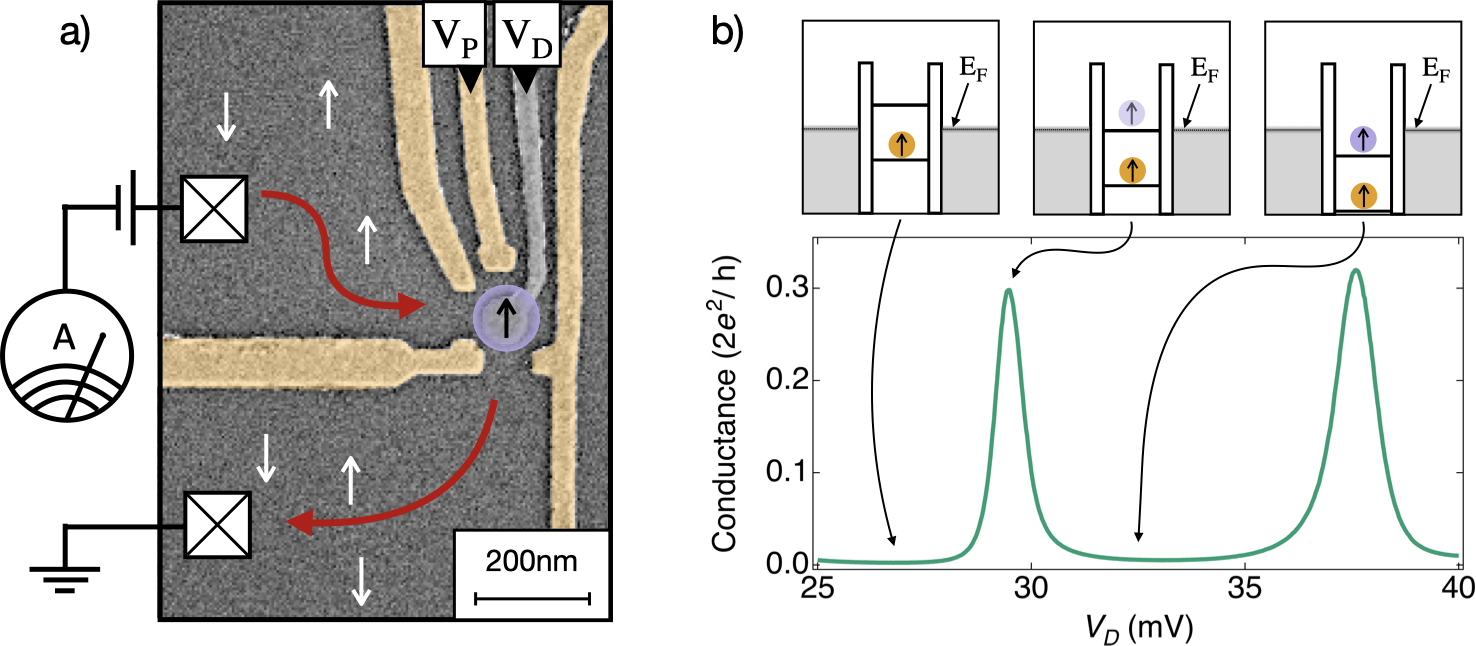
\includegraphics[width=1.0\textwidth]{figures/ch1/crop_PosterFiguresMaster.003.png}
    \caption[Conductance through a quantum dot]{\label{fig:ch1/dot_intro} 
    % For some options that work with pdf\LaTeX, please see this discussion:
    %   \url{http://tex.stackexchange.com/questions/11839}.  
    (\textbf{a}) an SEM image of the gates used to define a quantum dot. The gold coloured gates indicate sufficient negative potential is applied so that the 2DEG below is depleted. The gates V\textsubscript{P} or V\textsubscript{D} have the biggest effect on dot energy without changing other energies. The crossed are ohmic contacts which contact the 2DEG. By applying a small bias we measure the conductance through the quantum dot. (\textbf{b}) are Coulomb blockade energy diagrams illustrating how the conductance varies as an electron enters the quantum dot. The grey boxes represent the continuous energy level of electrons in the leads. The white rectangles represent tunnel barriers into and out-of the quantum dot. The rate of tunneling is described by the parameter $\Gamma$, the wider (narrower) the barrier, the smaller (larger) the rate of tunneling. (\textbf{c}) is a measurement showing the conductance through a quantum dot as a single electron (in purple) is added. From left to right: Electrons in the leads cannot tunnel into the quantum dot as there is no available energy level and hence we measure zero conductance. As V\textsubscript{D} is made less negative, the dot energy lowers and electrons can tunnel into the dot and back out. We measure a maximum in conductance when the dot energy is aligned with the leads. Once the dot energy falls below the level of the leads there is again no available energy level and the dot is insulating. 
      }
  \end{center}
\end{figure}

A quantum dot is formed by applying negative voltages to confine a small region in the 2DEG Fig.~\ref{fig:ch1/dot_intro}\textbf{a}.
Each of the gates near the quantum dot are capacitively coupled to the different parameters that determine the different energies in the dot. However, the gates geometry was designed for certain gates to affect some energies more than others. In Fig.~\ref{fig:ch1/dot_intro}\textbf{a}, $\mathrm{V_{LC}}$ is the 'left-coupling' gate and the strongest effect on the left tunnel barrier along with $\mathrm{V_{N}}$. $\mathrm{V_{N}}$ is the 'nose' gate and effects both coupling equally, it also has a large effect on the dot energy and can push the location of the electron wave function closer to $\mathrm{V_{CSS}}$. $\mathrm{V_{CSS}}$ is the 'charge sensor spine' the charge sensor is discussed in the next section but it is important for the wavefunction of the electron to be close to $\mathrm{V_{CSS}}$ for higher sensitivity of the charge sensor. $\mathrm{V_{P}}$ is the 'plunger' and is used primarily to control the dot energy as it is far from the tunnel barriers. By making this gate less negative the dot energy decreases and at some point another electron can enter the dot. $\mathrm{V_{D}}$ is the 'dot' gate, this gate is operated different to the other gates as it lies right above where the dot lives. This gate is most strongly coupled to the dot energy and we use this gate to add or remove single electrons into the quantum with fine control. This gate is normally at positive voltage values to help form the potential well as negative voltages will form a donut shaped potential. 



\afterpage{\clearpage}
\subsection{Charge Sensing a Quantum Dot}

\begin{figure}[!htb]
  \begin{center}
%% includegraphics: comment the following if not using the graphicx package
    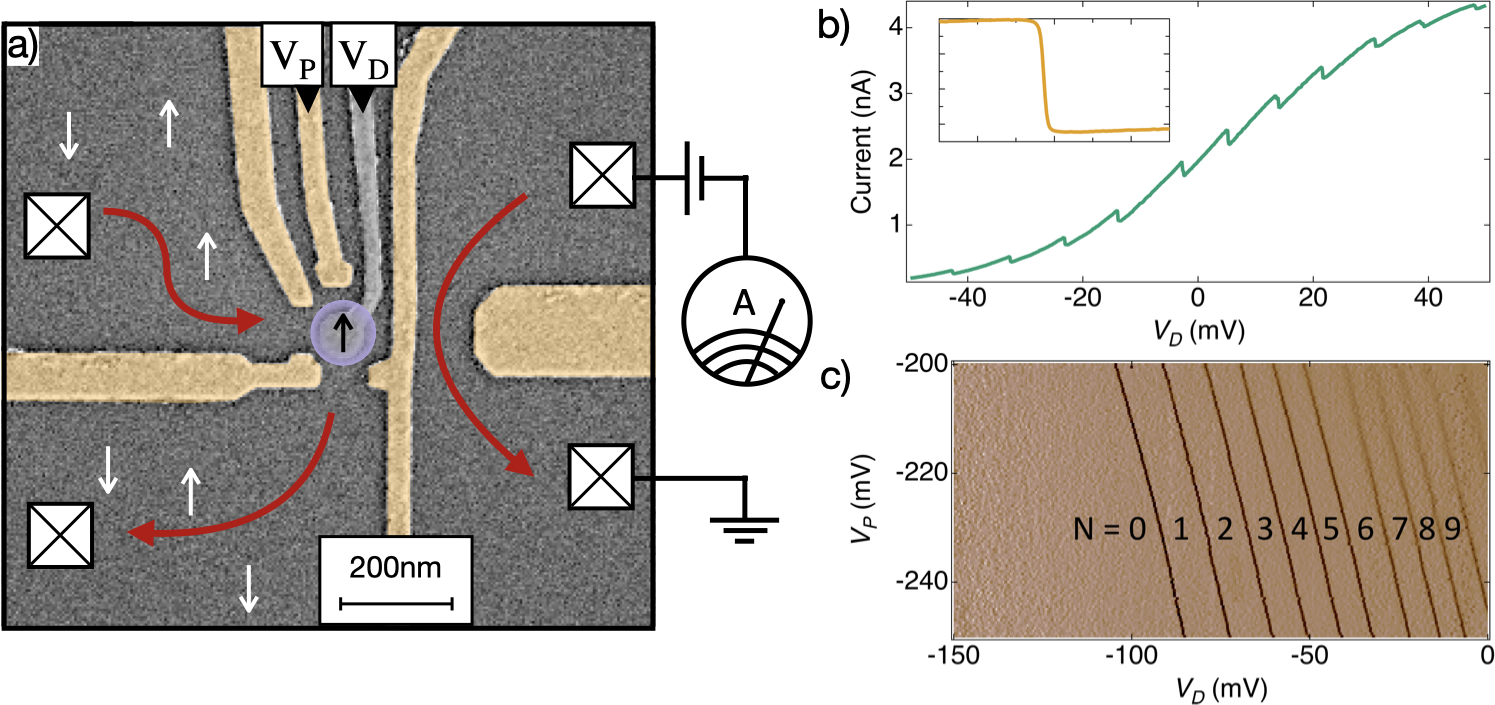
\includegraphics[width=1.0\textwidth]{figures/ch1/crop_PosterFiguresMaster.004.png}
    \caption[Charge sensing a quantum dot]{\label{fig:ch1/ct_intro} 
    % For some options that work with pdf\LaTeX, please see this discussion:
    %   \url{http://tex.stackexchange.com/questions/11839}.  
    (\textbf{a}) An SEM image of the gates used to define a quantum dot. The gold coloured gates indicate sufficient negative potential is applied so that the 2DEG below is depleted. The gates V\textsubscript{P} or V\textsubscript{D} have the biggest effect on dot energy without changing other energies. The crossed are ohmic contacts which contact the 2DEG. V\textsubscript{CSQ} is used to form a QPC near the quantum dot. By setting up the QPC on a steep slope the current through the QPC is sensitive to nearby changes in charge. (\textbf{b}) measuring the current across the charge sensing QPC. As V\textsubscript{D} becomes less negative the current through the QPC increases. The downward jumps in current are a result of the negative repulsion from electrons entering the quantum dot. The subfigure (yellow) shows a zoomed in scan over one of these transitions. (\textbf{c}) A 2d map showing how the occupation of the quantum dot changes as a function of V\textsubscript{P} and V\textsubscript{D}. The data is the differentiated current through the charge sensor. The differentiated steep slopes of the charge transitions show up as sharp peak which is useful for locating charge transitions when there is a large change in background current. 
      }
  \end{center}
\end{figure}

A charge sensor is a way to measure the charge around the quantum dot and if correctly tuned it is very sensitive to the additional charge of an electron that enters a quantum dot. It is formed by adding a QPC in close proximity to the quantum dot Fig.~\ref{fig:ch1/dot_intro}\textbf{a}. A QPC can be tuned to have a steep slope or plateau  Fig.~\ref{fig:ch1/qpc_intro}\textbf{c}. When used as a charge sensor, the QPC is tuned to be on a steep slope. This is useful as small changes in nearby potentials (x-axis of a QPC trace) show up as large changes in the current measured through the QPC. In Fig.~\ref{fig:ch1/dot_intro}\textbf{b} the QPC is set up on a steep slope and V\textsubscript{D} is swept from negative to positive to lower the dot energy so that electrons can hop in. The background increase in current is due to the capacitive coupling of V\textsubscript{D} as it is swept to more positive values. But once an electron can hop into the quantum dot the extra negative charge shows up as a small but sharp decrease in current which we call a 'charge transition'. The derivative of the current is useful for quickly identifying electrons entering the quantum dot as the steep slope of the charge transition shows up as a large negative spike. One of the functions of the charge sensor is to count how many electrons are in the quantum dot Fig.~\ref{fig:ch1/dot_intro}\textbf{c}. By making V\textsubscript{D} more negative whilst keeping the tunnel barrier open for electrons to enter the quantum dot we will at some point stop seeing charge transitions signalling the last electron. Also, a 2d sweep with a different gates on either axis tells us the relative cross capacitance between each gate on the dot energy. From Fig.~\ref{fig:ch1/dot_intro}\textbf{c}, a \qty{-50}{mV} change on V\textsubscript{D} remove $\sim~4$ electrons but \qty{-50}{mV} change on V\textsubscript{P} only removes $\sim~2$ electrons.



\afterpage{\clearpage}
\section{Electron Temperature from Charge Transitions}

\begin{figure}[!htb]
  \begin{center}
%% includegraphics: comment the following if not using the graphicx package
    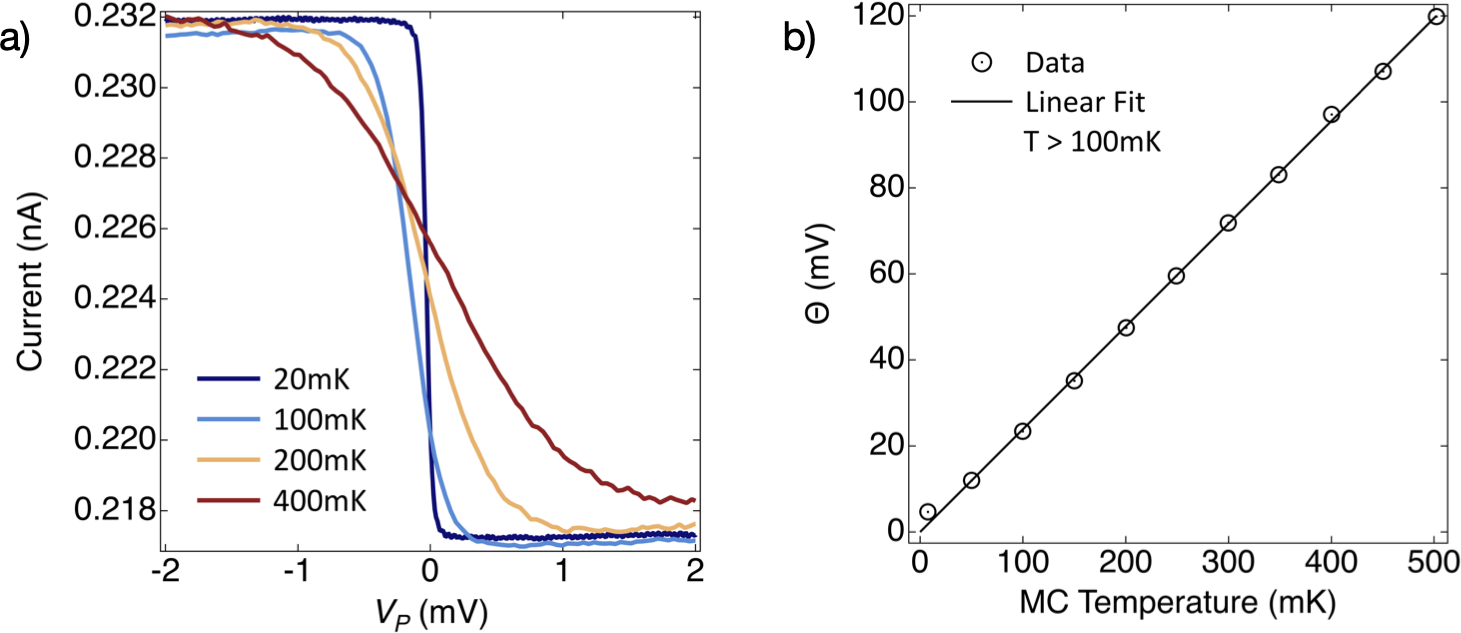
\includegraphics[width=1.0\textwidth]{figures/ch1/crop_PosterFiguresMaster.005.png}
    \caption[Calculating the electron temperature]{\label{fig:ch1/electron_temp} 
    % For some options that work with pdf\LaTeX, please see this discussion:
    %   \url{http://tex.stackexchange.com/questions/11839}.  
    (\textbf{a}) A weakly coupled charge transition measured at different fridge temperatures. The broadening of a weakly coupled charge transition is linearly proportional to its temperature. (\textbf{b}) A plot of the calculated broadening ($\Theta$) of the charge transition at different fridge temperatures. At fridge temperatures \qty{>100}{mK}, the increase in the charge transition broadening is linear. This indicates the electrons are well thermalised to the fridge. A linear fit to fridge temperatures \qty{>100}{mK} is extrapolated to base temperature to calculate the temperature of the electrons given the measure broadening. 
      }
  \end{center}
\end{figure}

Measuring charge transitions with the charge sensor lets us count the number of electrons in the quantum dot or the relative cross capacitance between different gates on the dot energy. But it can also be used to measure the temperature of the electrons in the 2DEG. When the broadening of a charge transition is due to the thermal energy of the system rather than the coupling strength to the source and drain leads ($\Gamma/\mathrm{T} << \mathrm{k_B T}$), the charge transition is described as being temperature broadened. The current through the charge sensor for a temperature broadened (weakly coupled) charge transition has lineshape,

\begin{equation}\label{eq:cs_lineshape}
  \mathrm{I_{CS}} = 
  \mathrm{I_{amp}}
  \tanh
  \left( 
  \frac{\mathrm{V_P - V_{mid}}}{2\Theta}
  \right) + 
  \gamma \mathrm{V_P}
  + \mathrm{I_{const}}
\end{equation}

where $\mathrm{I_{CS}}$ is the current through the charge sensor. $\mathrm{I_{amp}}$ is the amplitude of the charge transition, $\mathrm{V_{P}}$ is the voltage on the sweep gate to sweep over the charge transition, $\mathrm{V_{mid}}$ is the mid point of the charge transition. $\Theta=\frac{\mathrm{k_B}T}{\mathrm{\alpha e}}$ is the thermal broadening in units of gate voltage, where $\alpha \equiv \frac{\mathrm{d\epsilon}}{\mathrm{dV_P}}$ is a leverarm that relates changes in a gate voltage to changes in the dot energy. $\gamma$ is the cross capacitance between the sweep gate and the current through the charge sensor. $\mathrm{I_{const}}$ is a constant current offset.

The broadening of a temperature broadened charge transition can be used to determine the temperature of the electrons in thee 2DEG as the broadening is linearly proportional to the temperature ($\Theta\propto\mathrm{T}$) of the electrons Fig.~\ref{fig:ch1/electron_temp}\textbf{a}. At high fridge temperatures, the electrons in the 2DEG are in thermal equilibrium with the fridge. But as the fridge reaches base temperature (\qty{7}{mK}), the electrons in the 2DEG will not be in equilibrium due to poor thermal contact and source drain biases that can heat the electrons (i.e. \qty{1}{\mu eV}~=~\qty{11.6}{mK}). 
% Also charge noise that shifts the charge transition left or right in gate space 
To determine the proportionality constant between the broadening and temperature, charge transitions are measured at a range of fridge temperatures from \qty{8}{}~-~\qty{500}{mK}. Each charge transition will be measured quickly ($\sim$\qty{0.5}{s}) and repeated many times ($\sim300$). Any traces with large jumps in current near the charge transition ('charge jumps') are thrown out, and the remaining traces are then centered and averaged. The quick scans and averaging reduces additional broadening that come from charge motion in the dopant layer which shifts the charge transition left and right. The amount charge motion in the dopant layer scales between $\mathrm{1/f}$ and $\mathrm{1/f^2}$ [XXX]. Each charge transition is then fit using Eq.~\ref{eq:cs_lineshape} and the calculated $\Theta$ is plotted versus the fridge temperature Fig.~\ref{fig:ch1/electron_temp}\textbf{b}. A linear fit to $\Theta$ between \qty{100}{}~-~\qty{500}{mK} determines the proportionality constant. This is then used to convert the $\Theta$ measured as base temperature into the effective temperature of the electrons in the 2DEG. In this fridge we determine a base electron temperature of \qty{20}{mK}.


\subsection{Charge Sensing with a Virtual Gate}

\begin{figure}[!htb]
  \begin{center}
%% includegraphics: comment the following if not using the graphicx package
    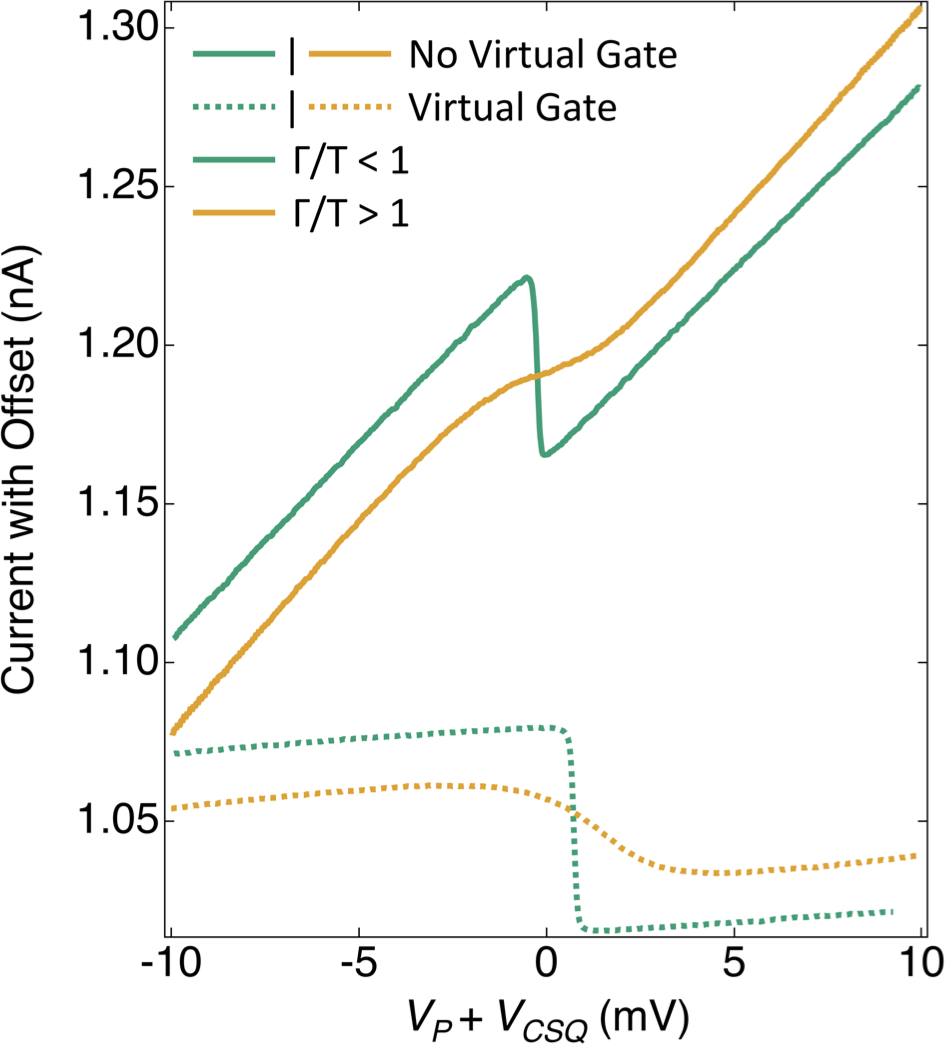
\includegraphics[width=0.8\textwidth]{figures/ch3/crop_PosterFiguresMaster.009.png}
    \caption[Measuring charge transitions with and without a virtual gate]{\label{fig:ch3/virtual_gate_example} 
    % For some options that work with pdf\LaTeX, please see this discussion:
    %   \url{http://tex.stackexchange.com/questions/11839}.  
    Data of a weakly (green) and strongly (yellow) coupled charge transition scanned with a single gate V\textsubscript{P} (solid line) and a virtual gate  V\textsubscript{P}~+~V\textsubscript{CSQ} (dashed line). The traces have been offset in current for ease of comparison. V\textsubscript{P} has a large effect on the dot energy, however, it also changes other parameters due to capacitive coupling. Here, a virtual gate is used to change the dot energy whilst keeping the current through the charge sensor constant. This helps with visually identifying strongly coupled charge transitions which become very broadened. More importantly, the charge sensor stays in the linear regime where changes in the potential are linearly proportional to changes in the current. Note the x-axis is only showing the value of V\textsubscript{P}. As V\textsubscript{P} is swept negative to positive, V\textsubscript{CSQ} is swept positive to negative.}
  \end{center}
\end{figure}


Temperature broadened transitions are straightforward to fit as they are described by an analytic function where the broadening is due to a single parameters and the sharpness of the transitions makes visual inspection of the fits trivial. The work in this thesis focuses on coupling strengths of $\Gamma/\mathrm{T}>1$. The charge transition at these larger coupling strengths becomes very spread out and it can be tricky to visually inspect the quality of the fits. 

One way to tackle this problem is by using a virtual gate. In general, a virtual gate is a name give to a combination of gates that when varied, change a parameter of the dot whilst keeping other parameters constant. The main parameters we think about are the dot energy $\mathrm{\epsilon}$, left coupling $\mathrm{\Gamma_L}$, right coupling $\mathrm{\Gamma_R}$ and current through the charge sensor $\mathrm{I_{CS}}$. An example usage would be a virtual gate that controls the left coupling $\mathrm{\Gamma_L}$ only. A combination of V\textsubscript{LC} and V\textsubscript{P} would be used. V\textsubscript{LC} to primarily changed the left coupling $\mathrm{\Gamma_L}$ and V\textsubscript{P} to offset any changes to the dot energy. 

In the context of this thesis, only a virtual gate that changes the dot energy but keeps the current constant through the charge sensor is used. Fig.~\ref{fig:ch3/virtual_gate_example} shows the effect of this virtual gate on a weakly coupled ($\Gamma/\mathrm{T}<1$) and strongly coupled ($\Gamma/\mathrm{T}>1$) charge transition. By sweeping V\textsubscript{CSQ} in the opposite direction of V\textsubscript{P}, the cross-capacitive effect of V\textsubscript{P} on the charge sensor is largely removed. 


\afterpage{\clearpage}
\section{Measurement Pocedures}

\subsection{Cooldown Bias}
At room temperature, $+$\qty{200}{mV} is applied to all the gates forming the dot and charge sensor (apart from V\textsubscript{D}). This positive bias repels the postive charge underneath the gates in the dopant layer. Once the device reaches \qty{10}{K}, the dopants are frozen in and an effective potential is seen by the electrons in the 2DEG due to the absence of positive charge. Cooling with bias has two advantages. One, it reduces the charge noise [XXX]. Two, it reduces the amount of negative potential required on the gates. The effective potential from the positive bias is roughly equal to a negative bias of equal magnitude when the device is cold (i.e. $+$\qty{200}{mV} cooldown bias $\approx$ $-$\qty{200}{mV}). This is useful as the fine gates can 'blow-up' (in reality the metal gates will lift off a little from the heterostructure surface) from high voltages rendering the device un-measurable. The fine gates are also sensitive to static discharge, so we put \qty{1}{M\Omega} of inline resistance on all of the gates.   

\subsection{Gate Dividers}
When measuring charge transitions with a virtual gate we often require fine gate control at large voltages. For example, V\textsubscript{P} may need a voltage of $-$\qty{500}{mV} but a resolution of \qty{0.001}{mV}. Digital-to-analog converter (DAC) channels are used to apply the voltage on the gates. The DACs have a range of $\pm$\qty{10}{V}, with 16-bit resolution. This puts a lower bound on the step size of \qty{0.305}{mV} ($\mathrm{\qty{20}{V}/2^{16}}$). To achieve achieve the large voltage range with high resolution, two DACs are connected to the same gate. One DAC channel is used to cover a wide voltage range whilst the other is used for fine control by adding a voltage divider in-line. Voltage dividers between $20$ and $100000$ are commonly used to achieve the required resolution (up to \qty{3}{nV}). All of the voltages in this thesis have been converted to the real voltage applied to the gate (i.e. not the voltage output on the DAC). However, we commonly use the fine gate to sweep over transitions and do not show the rough gate voltage that is also applied to the same gate for clarity. 




 




